\documentclass[11pt,a4paper]{article}

% ---------------------------------------------------------------- packages
\usepackage[margin=2.3cm]{geometry}
\usepackage[T1]{fontenc}
\usepackage{mathptmx}
\usepackage{microtype}
\usepackage{booktabs}
\usepackage{array}
\usepackage{tabularx}
\usepackage{multirow}
\usepackage{enumitem}
\usepackage{xcolor}
\usepackage{caption}
\usepackage{float}
\usepackage{pgfplots}
\pgfplotsset{compat=1.18}
\usepackage[hidelinks]{hyperref}

\setlist{nosep,leftmargin=*}
\emergencystretch=2em
\captionsetup{font=small,labelfont=bf}
\definecolor{ours}{RGB}{31,111,196}
\definecolor{paper}{RGB}{150,150,150}
\newcommand{\pass}[1]{\texttt{#1}}

\title{\textbf{OS-Sanitizer: Artifact Verification, Benchmarking\\and Report Clustering}\\[4pt]
\large Project report: an extension of OS-Sanitizer}
\author{Pradeep Kumar Mahato (26954) \and Vivek Kumar (26357)}
\date{November 2026}

\begin{document}
\maketitle

% ================================================================ abstract
\begin{abstract}
OS-Sanitizer~\cite{ossan} uses eBPF to infer latent defects in Linux applications from benign
runtime behaviour. Its authors left two problems open: reports are heavily duplicated, and no
false-positive rate could be computed because whether a report is real depends on execution context.
We reproduced the public artifact~\cite{artifact} on a Fedora~39 virtual machine and verified it:
the artifact builds cleanly, all 15 passes detect their reference programs, and the paper's
Tables~2 and~3 regenerate exactly from the shipped data. Re-measured microbenchmark overheads
(10+10 runs per pass) show the same ranking and order of magnitude as the paper, and on five real
workloads every individual non-memory pass stays within 7\% except \pass{filep\_unlocked} on
\texttt{gcc} (1.30$\times$; paper 1.32$\times$). We found and fixed a bug that made the
\pass{memcpy} pass blind on CPUs without the ERMS feature, and found a second bug in which enabling
\pass{intercept\_path} suppresses \pass{sec\_file\_open} reports. We then extended every report with
credentials, executable identity and file ownership captured in the kernel, written as JSON, and
added automated clustering. A 13.4-hour system-wide capture produced 207{,}854 reports in 1{,}910
clusters; the 79{,}091 ERROR/WARN reports collapse to 1{,}034 clusters. A preliminary,
transparent scoring method reached precision 1.00 and recall 0.80 on 33 labelled scenarios across
nine passes.
\end{abstract}

% ================================================================ 1
\section{Introduction}

OS-Sanitizer brings the idea of code smells into dynamic testing. Instead of waiting for a program
to fail, it watches benign behaviour system-wide with eBPF and reports patterns that could become
defects in another context. Over a month on a developer laptop it led to more than 40 confirmed
issues, including in Go, Docker and PCRE2~\cite{ossan}.

The paper leaves two problems open:
\begin{itemize}
  \item \textbf{Duplicate reports.} Each suspicious \emph{event} produces a report, so one code
  location is reported many times: on average 244 log entries per unique stack-trace offset
  (Section~6.4.2 of~\cite{ossan}). The authors deduplicated by hand and note that automated
  aggregation is possible (Takeaway~\#4).
  \item \textbf{No false-positive rate.} The same code is safe in one context and exploitable in
  another (Section~2, Scenarios~1--3). Severity levels depend only on the kind of action, so they
  cannot express this (Section~8.2).
\end{itemize}

This project verifies the published results on independent hardware and builds the first stage of
the false-positive calibration layer we proposed: kernel-captured context and automated
deduplication. Our contributions are:
\begin{enumerate}
  \item reproduction and verification of the artifact, including both overhead tables
  (Sections~\ref{sec:verify}--\ref{sec:bench});
  \item two artifact bugs, one fixed (Section~\ref{sec:bugs});
  \item context-enriched JSON reports captured in the kernel (Section~\ref{sec:ctx});
  \item automated report clustering evaluated on a 13.4-hour real-system capture
  (Section~\ref{sec:cluster});
  \item a preliminary, transparent scoring method evaluated on labelled scenarios
  (Section~\ref{sec:score}).
\end{enumerate}

% ================================================================ 2
\section{Background}

OS-Sanitizer consists of 15 \emph{passes}. A pass is a group of eBPF programs attached to kernel
functions (fentry/fexit), userspace library functions (uprobes) or Linux Security Module hooks,
which share state through eBPF maps and send a report to a userspace launcher when a defect pattern
occurs. Table~\ref{tab:passes} lists the passes in the paper's four classes.

\begin{table}[H]
\centering\small
\caption{OS-Sanitizer passes (Section 4.2 of~\cite{ossan}).}
\label{tab:passes}
\begin{tabularx}{\linewidth}{@{}>{\raggedright}p{2.6cm} >{\raggedright}p{4.4cm} >{\raggedright\arraybackslash}X@{}}
\toprule
Class & Passes & Reports when \\
\midrule
System interactions & \pass{access}, \pass{fixed\_mmap}, \pass{rwx\_mem} & stat/access before open (TOCTOU), unsafe \texttt{MAP\_FIXED}, writable+executable memory \\
Library usage & \pass{filep\_unlocked}, \pass{gets}, \pass{snprintf}, \pass{printf\_mut}, \pass{system\_mut}, \pass{system\_abs} & unsynchronised \texttt{FILE*} use, \texttt{gets()}, snprintf length misuse, non-constant format strings or commands, relative command paths \\
Environmental & \pass{sec\_file\_open}, \pass{intercept\_path} & opening world-writable files; paths other users can redirect \\
Memory functions & \pass{memcpy}, \pass{strcpy}, \pass{strncpy}, \pass{sprintf} & copies into stack buffers whose length depends on input \\
\bottomrule
\end{tabularx}
\end{table}

The launcher resolves each report's stack trace, applies a few hard-coded filters and assigns a
fixed severity per pass and action type: ERROR (e.g.\ root executing a user-writable file), WARN, or
INFO (e.g.\ a stat-then-open pattern). In the paper's long-term study, analysts read only ERROR and
WARN reports, about two hours per week, and judged each by hand. Severity describes the \emph{kind}
of action, not \emph{who could exploit it}: the same TOCTOU pattern is INFO whether root runs it on
its own files (safe) or in a directory another user controls (exploitable).

% ================================================================ 3
\section{Experimental setup}

All experiments ran on one Fedora~39 virtual machine, the same distribution as the paper's
systems, using the artifact at commit \texttt{aad89c1} (Table~\ref{tab:setup}). Early functional
checks ran on the same VM with 6~vCPUs before it was resized; all benchmark numbers come from the
10-vCPU configuration. Table~\ref{tab:data} lists the data sets.

\begin{table}[H]
\centering\small
\caption{Experimental platform.}
\label{tab:setup}
\begin{tabularx}{\linewidth}{@{}l X X@{}}
\toprule
& This work & Paper, System A~\cite{ossan} \\
\midrule
OS / kernel & Fedora 39, kernel 6.11.9-100.fc39 & Fedora 39 \\
Hardware & VirtualBox VM (KVM paravirtualisation), 10 vCPU AMD Ryzen 5 5600G, 22~GiB & KVM VM, 4 vCPU Intel Xeon Gold 6248R, 24~GiB \\
Toolchain & Rust nightly 1.102, bpf-linker 0.11.1, clang 17.0.6, gcc 13.3.1, glibc 2.38 & not stated \\
\bottomrule
\end{tabularx}
\end{table}

\begin{table}[H]
\centering\small
\caption{Data sets.}
\label{tab:data}
\begin{tabularx}{\linewidth}{@{}l X l@{}}
\toprule
Data set & Content & Section \\
\midrule
Microbenchmarks & The artifact's 15 example programs in a 10-second loop; 10 runs with and 10 without OS-Sanitizer per pass & \ref{sec:micro} \\
Real workloads & \texttt{xz}, \texttt{gcc}, \texttt{perl}, \texttt{sqlite3}, \texttt{stockfish} (stand-ins for the licensed SPEC CPU~2017); 5 runs per configuration (hyperfine) & \ref{sec:real} \\
System-wide capture & \texttt{-{}-reference-policy} (12 passes) as a systemd service, 13.4~h of normal development use (2026-11-11 13:26 to 2026-11-12 02:51), 569~MiB JSON & \ref{sec:volume}, \ref{sec:cluster} \\
Labelled scenarios & 33 constructed safe/exploitable scenarios over 9 passes, 457 reports & \ref{sec:score} \\
\bottomrule
\end{tabularx}
\end{table}

% ================================================================ 4
\section{Artifact verification}
\label{sec:verify}

Every check in Table~\ref{tab:verify} passed, once the \pass{memcpy} pass was fixed
(Section~\ref{sec:bugs}). The binding check matters because aya-based eBPF programs read kernel
structures at fixed offsets; a mismatch would not fail loudly but silently produce wrong uids,
modes or paths.

\begin{table}[H]
\centering\small
\caption{Artifact verification.}
\label{tab:verify}
\begin{tabularx}{\linewidth}{@{}l X X@{}}
\toprule
Check & Method & Result \\
\midrule
Build & \texttt{cargo build --release} from source & Clean in 1~min 24~s; byte-identical to the separately installed binary \\
Kernel struct layouts & Regenerated \texttt{binding.rs} with \texttt{aya-tool} and compared & Identical to the shipped file \\
Paper tables from shipped data & Authors' scripts in \texttt{evaluation/output/} & Table 2 reproduced exactly; Table 3 regenerates with its significance tests \\
Detection & Each pass alone, its example program run once & 15 of 15 passes report their example \\
Report contents & Inspected file-pass reports & Paths, permission bits and writer lists correct \\
\bottomrule
\end{tabularx}
\end{table}

% ================================================================ 5
\section{Benchmarking}
\label{sec:bench}

\subsection{Microbenchmarks (paper Table 2)}
\label{sec:micro}

Each example program executes exactly the pattern its pass reports, in a tight loop for 10~seconds.
Table~\ref{tab:t2} and Figure~\ref{fig:t2} compare the median time per iteration with the paper.
The ranking is the same: the four userspace memory passes and the printf-family passes cost
24--159$\times$ in this worst case, the system-call passes 1--10$\times$. Our ratio is within
1.6$\times$ of the paper's for every pass except \pass{memcpy}, whose instrumented call costs
3.5~$\mu$s here against 10.0~$\mu$s in the paper.

\begin{table}[H]
\centering\small
\caption{Microbenchmarks: iteration time in $\mu$s (median of 10 runs) and overhead ratio.}
\label{tab:t2}
\begin{tabular}{@{}l rrr rrr@{}}
\toprule
& \multicolumn{3}{c}{This work} & \multicolumn{3}{c}{Paper~\cite{ossan}} \\
\cmidrule(lr){2-4}\cmidrule(l){5-7}
Pass & Baseline & OS-San. & Ratio & Baseline & OS-San. & Ratio \\
\midrule
\pass{access}         & 3.63    & 15.38   & 4.24   & 1.98    & 7.33    & 3.70 \\
\pass{fixed\_mmap}    & 9.59    & 53.87   & 5.62   & 7.19    & 27.05   & 3.76 \\
\pass{rwx\_mem}       & 5.06    & 48.15   & 9.52   & 2.55    & 15.22   & 5.96 \\
\pass{filep\_unlocked}& 6.78    & 9.68    & 1.43   & 3.55    & 6.07    & 1.71 \\
\pass{gets}           & 78.64   & 110.05  & 1.40   & 54.10   & 60.69   & 1.12 \\
\pass{snprintf}       & 0.33    & 9.37    & 28.43  & 0.28    & 6.81    & 24.04 \\
\pass{printf\_mut}    & 0.25    & 8.08    & 31.72  & 0.18    & 6.33    & 34.94 \\
\pass{system\_mut}    & 2160.99 & 2244.42 & 1.04   & 4571.43 & 4905.57 & 1.07 \\
\pass{system\_abs}    & 2173.44 & 2253.78 & 1.04   & 4465.28 & 4916.42 & 1.10 \\
\pass{sec\_file\_open}& 2.81    & 5.07    & 1.81   & 1.38    & 3.22    & 2.33 \\
\pass{intercept\_path}& 3.08    & 14.93   & 4.84   & 1.53    & 6.13    & 4.00 \\
\midrule
\pass{memcpy}         & 0.05    & 3.46    & 63.47  & 0.07    & 9.96    & 140.19 \\
\pass{strcpy}         & 0.05    & 4.65    & 95.89  & 0.04    & 4.68    & 106.38 \\
\pass{strncpy}        & 0.06    & 10.26   & 159.24 & 0.09    & 9.46    & 103.90 \\
\pass{sprintf}        & 0.08    & 5.15    & 67.95  & 0.10    & 4.77    & 46.56 \\
\bottomrule
\end{tabular}
\end{table}

\begin{figure}[H]
\centering
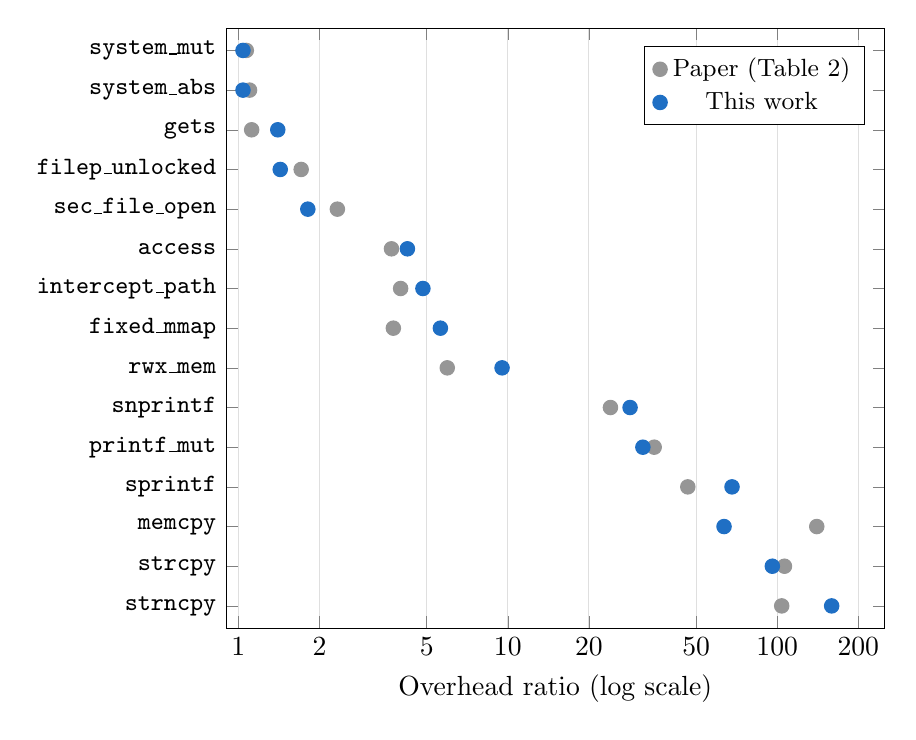
\begin{tikzpicture}
\begin{axis}[
  width=0.82\linewidth, height=9.2cm,
  xmode=log, xmin=0.9, xmax=250,
  xlabel={Overhead ratio (log scale)},
  log ticks with fixed point,
  xtick={1,2,5,10,20,50,100,200},
  symbolic y coords={system\_mut,system\_abs,gets,filep\_unlocked,sec\_file\_open,access,intercept\_path,fixed\_mmap,rwx\_mem,snprintf,printf\_mut,sprintf,memcpy,strcpy,strncpy},
  ytick=data, y dir=reverse,
  yticklabel style={font=\small\ttfamily},
  xmajorgrids, grid style={gray!25},
  legend style={at={(0.97,0.97)},anchor=north east,font=\small},
  enlarge y limits=0.04,
]
\addplot[only marks, mark=*, mark size=2.6pt, color=paper] coordinates {
 (1.07,system\_mut) (1.10,system\_abs) (1.12,gets) (1.71,filep\_unlocked) (2.33,sec\_file\_open)
 (3.70,access) (4.00,intercept\_path) (3.76,fixed\_mmap) (5.96,rwx\_mem) (24.04,snprintf)
 (34.94,printf\_mut) (46.56,sprintf) (140.19,memcpy) (106.38,strcpy) (103.90,strncpy)};
\addplot[only marks, mark=*, mark size=2.6pt, color=ours] coordinates {
 (1.04,system\_mut) (1.04,system\_abs) (1.40,gets) (1.43,filep\_unlocked) (1.81,sec\_file\_open)
 (4.24,access) (4.84,intercept\_path) (5.62,fixed\_mmap) (9.52,rwx\_mem) (28.43,snprintf)
 (31.72,printf\_mut) (67.95,sprintf) (63.47,memcpy) (95.89,strcpy) (159.24,strncpy)};
\legend{Paper (Table 2), This work}
\end{axis}
\end{tikzpicture}
\caption{Microbenchmark overhead per pass, this work vs.\ the paper.}
\label{fig:t2}
\end{figure}

\subsection{Real workloads (paper Table 3)}
\label{sec:real}

SPEC CPU~2017 is licensed and takes days to run, so we used five freely available programs with
similar character. Each configuration is compared with baselines measured immediately before and
after it (one-sided Welch's $t$-test, $p<0.05$). As in the paper, the non-memory passes add
little overhead: apart from \pass{filep\_unlocked} on \texttt{gcc} (1.30$\times$; paper
1.32$\times$, caused by gcc's exclusive use of unlocked file I/O), no individual pass exceeds
7\%. The memory passes are expensive on string-heavy workloads: \pass{memcpy}, \pass{strcpy} and
\pass{strncpy} each slow \texttt{sqlite3} by about 4.3$\times$. These three share the same
\texttt{strlen} probes, which explains their near-identical cost.

\begin{table}[H]
\centering\small
\caption{Overhead ratio over baseline on real workloads. \textbf{Bold}: significant at $p<0.05$.
Workloads are stand-ins for the SPEC benchmark named in brackets.}
\label{tab:t3}
\begin{tabular}{@{}l ccccc@{}}
\toprule
Pass & xz & gcc & perl & sqlite & stockfish \\
 & \footnotesize(657.xz) & \footnotesize(602.gcc) & \footnotesize(600.perlbench) & \footnotesize(620.omnetpp) & \footnotesize(631.deepsjeng) \\
\midrule
\pass{access}         & \textbf{1.02} & 1.00 & 1.00 & 1.02 & 1.00 \\
\pass{fixed\_mmap}    & 1.00 & 1.00 & 1.00 & 1.00 & 0.99 \\
\pass{rwx\_mem}       & 1.01 & 1.00 & 1.00 & 1.01 & 1.01 \\
\pass{filep\_unlocked}& 1.00 & \textbf{1.30} & 0.97 & \textbf{1.01} & 1.00 \\
\pass{gets}           & 1.00 & 1.01 & 1.00 & 0.97 & 1.01 \\
\pass{snprintf}       & 1.02 & \textbf{1.07} & \textbf{1.04} & 1.01 & 1.01 \\
\pass{printf\_mut}    & 1.00 & \textbf{1.02} & \textbf{1.02} & 1.03 & 1.01 \\
\pass{system\_mut}    & 1.00 & 1.00 & 1.01 & 1.00 & \textbf{1.01} \\
\pass{system\_abs}    & 1.01 & 1.00 & 1.01 & 1.01 & 1.02 \\
\pass{sec\_file\_open}& 1.00 & 0.99 & \textbf{1.01} & 1.00 & 1.01 \\
\pass{intercept\_path}& \textbf{1.00} & 0.99 & 1.00 & 1.01 & 1.00 \\
All previous          & 0.98 & \textbf{1.45} & \textbf{1.17} & \textbf{1.04} & \textbf{1.03} \\
\midrule
\pass{memcpy}         & 1.02 & \textbf{1.32} & \textbf{1.06} & \textbf{4.31} & \textbf{1.03} \\
\pass{strcpy}         & \textbf{1.04} & \textbf{1.32} & \textbf{1.05} & \textbf{4.32} & 1.01 \\
\pass{strncpy}        & 1.00 & \textbf{1.34} & \textbf{1.07} & \textbf{4.28} & \textbf{1.03} \\
\pass{sprintf}        & 1.01 & \textbf{1.06} & 1.00 & 1.01 & 0.99 \\
All passes            & \textbf{1.05} & \textbf{1.77} & \textbf{1.05} & \textbf{4.33} & \textbf{1.03} \\
\midrule
\emph{Baseline time [s]} & 19.87 & 19.89 & 6.57 & 8.96 & 13.48 \\
\bottomrule
\end{tabular}
\end{table}

\subsection{Report volume (paper Section 6.4.2)}
\label{sec:volume}

The system-wide capture reproduces the paper's observation that a few passes produce most reports
(Table~\ref{tab:volume}). \pass{access} alone produced 116k INFO reports and \pass{sprintf} 72.5k
WARN reports, while \pass{system\_mut} reported once and \pass{gets} 30 times.

\begin{table}[H]
\centering\small
\caption{Report volume of the system-wide capture compared with the paper.}
\label{tab:volume}
\begin{tabular}{@{}l r r@{}}
\toprule
Metric & This work & Paper~\cite{ossan} \\
\midrule
Collection period & 13.4 hours & 5 busiest days of 1 month \\
Reports (log entries) & 207{,}854 & about 679{,}000 \\
\quad of which ERROR / WARN / INFO & 68 / 78.5k / 129k & -- \\
Unique binary offsets in stack traces & 6{,}098 & 2{,}784 \\
Unique binaries & 243 & 127 \\
Entries per unique offset & 34 & 244 \\
\bottomrule
\end{tabular}
\end{table}

% ================================================================ 6
\section{Issues found in the artifact}
\label{sec:bugs}

\paragraph{\pass{memcpy} pass blind on CPUs without ERMS (fixed).}
The pass produced no report for its own example. It hooks glibc's internal memcpy variants by name,
but only the \texttt{\_erms} ones. glibc chooses a variant at load time from CPU features, and our
VM does not expose ERMS (Enhanced REP MOVSB), so glibc ran \texttt{\_\_memmove\_avx\_unaligned},
which was never hooked. We added the 20 non-ERMS variants to the launcher's attach list; a missing
symbol is skipped, so the change is safe on every CPU. After the fix the pass detects its example.
Virtual machines and cloud instances often hide ERMS, so on such systems both detection and the
measured overhead of this pass depend on a CPU feature the paper does not mention.

\paragraph{\pass{intercept\_path} suppresses \pass{sec\_file\_open} reports (open).}
With \texttt{-{}-security-file-open} alone, opening a world-writable file is reported; with
\texttt{-{}-interceptable-path} also enabled, only the \pass{intercept\_path} report appears. We
reproduced this with the original binary. Both passes attach programs to the kernel function
\texttt{security\_file\_open}; the exact cause is not yet located. Until it is fixed, the two
passes should be run separately when both report types matter.

\paragraph{Not a defect.} Some ICU hooks fail with ``error resolving symbol''. They target
version-72 symbol names; Fedora~39 ships ICU~73, whose hooks attach correctly.

% ================================================================ 7
\section{Context-enriched reports}
\label{sec:ctx}

Deciding whether a report is exploitable requires knowing who ran the code, with which privileges,
and who else controls the files involved. Most original report types carried only a 16-character
process name, a PID and a stack-trace id. Recovering the rest later from \texttt{/proc/<pid>} is
unreliable: short-lived processes are often gone, the launcher handles reports asynchronously,
PIDs are reused, and a later lookup is itself a time-of-check/time-of-use race. The process name is
also spoofable with \texttt{prctl(PR\_SET\_NAME)}.

Every report now carries the fields in Table~\ref{tab:ctx}, captured in the kernel at the moment of
the event, and a new \texttt{-{}-json FILE} option writes each report as one structured record.

\begin{table}[H]
\centering\small
\caption{Context captured in the kernel for every report.}
\label{tab:ctx}
\begin{tabularx}{\linewidth}{@{}l l X@{}}
\toprule
Field & Kernel source & Purpose \\
\midrule
uid/gid, euid/egid, fsuid/fsgid & \texttt{task->cred} & Real vs.\ effective privilege; setuid detection \\
Executable inode, device, owner, mode & \texttt{task->mm->exe\_file} & Unspoofable binary identity; root running a user-owned binary \\
Parent uid & \texttt{task->real\_parent->cred} & A less-privileged parent controls argv, environment, stdin \\
cgroup id, boot-time timestamp & eBPF helpers & Service or container; ordering, repetition \\
File and parent-directory owner/mode & \texttt{file->f\_inode}, \texttt{d\_parent} & Can another user replace the opened entry? \\
Untrusted-open flag & observe-only LSM hook on \texttt{file\_open} & Privileged process opened a file another user controls \\
\bottomrule
\end{tabularx}
\end{table}

The context is written into a reserved 128-byte tail of the existing 4~KiB report buffer inside the
shared \texttt{emit\_report} function, so every pass gets it without changing any report format.
Two engineering problems arose. A first version pushed the \pass{intercept\_path} program to
528~bytes of stack, over the kernel's 512-byte limit, and was rejected by the verifier; the context
is now built in a per-CPU map. Writing JSON initially halved the launcher's throughput because
every record resolved \texttt{/proc/<pid>/exe}; a per-(pid, inode) cache recovered most of it.
Kernel-side capture proved necessary in practice: for a report whose process had already exited,
the \texttt{/proc} lookup was empty, while the captured inode still identified the exact binary.

% ================================================================ 8
\section{Report clustering}
\label{sec:cluster}

\subsection{Motivation and design}

A human decides once per code location, not once per event. Clustering automates the manual
deduplication described in the paper, and it is required before any accuracy measurement: if
individual reports were labelled, one busy code location would count thousands of times and appear
in both training and test data. Clustering does not decide whether a report is real, so it needs no
ground truth and applies to all 15 passes.

Two reports share a cluster only if all four parts of the key in Table~\ref{tab:key} match. The
context signature distinguishes this from plain deduplication: without it, root running a
stat-then-open in its own directory and in a user-controlled directory would form one cluster, and
any label given to it would be wrong for half of its reports.

\begin{table}[H]
\centering\small
\caption{Cluster key.}
\label{tab:key}
\begin{tabularx}{\linewidth}{@{}l X@{}}
\toprule
Key part & Reason \\
\midrule
Pass & Different defect types stay separate; no cluster mixes passes \\
Executable identity (verified path, else kernel inode) & The same library code in two programs is used in two contexts \\
Top 5 stack frames as binary + file offset & Identifies the code location; file offsets are stable across runs, unlike ASLR-randomised addresses \\
Context signature & Privileged; entry replaceable by another user; other writers on the path; untrusted input opened \\
\bottomrule
\end{tabularx}
\end{table}

The stack depth of 5 was chosen on an early 2-minute capture of 3{,}566 reports: 1 frame gave 22
clusters, 3 gave 39, 5 gave 50 and 7 gave 57. Fewer frames merge different call sites; more frames
split one call site by the path that reached it.

\subsection{Results}

On the 13.4-hour capture, clustering reduced 207{,}854 reports to 1{,}910 clusters (109 reports per
cluster). The 79{,}091 ERROR and WARN reports, the ones the paper's analysts read, fall into 1{,}034
clusters, a 77-fold reduction. Figure~\ref{fig:clusters} shows the reduction per pass. Cluster sizes
are highly skewed: the median cluster holds 3 reports, 522 clusters hold one, and the largest holds
24{,}920, a single TOCTOU call site in the VS~Code remote server's runtime that one decision covers.

\begin{figure}[H]
\centering
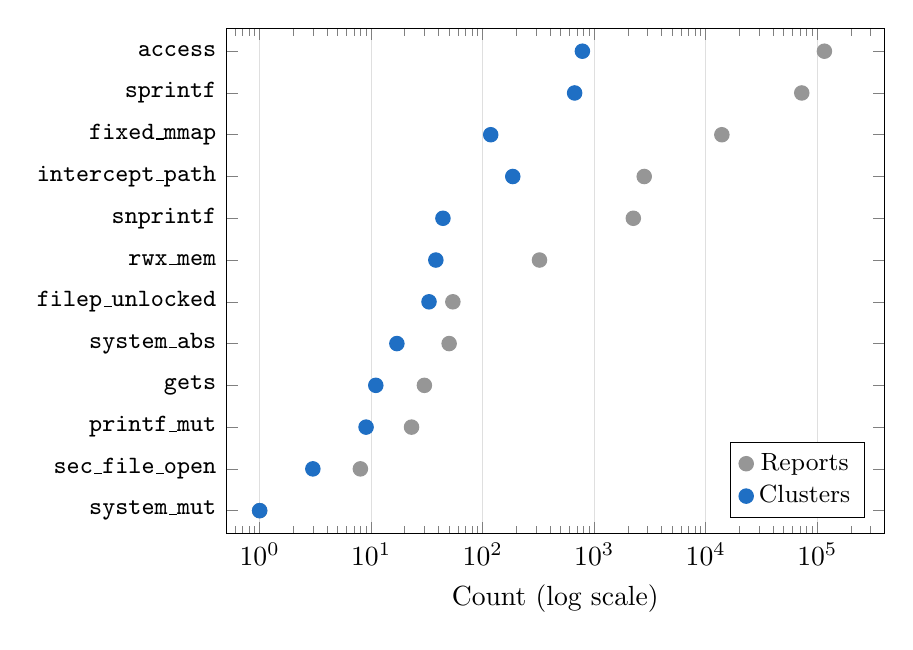
\begin{tikzpicture}
\begin{axis}[
  width=0.82\linewidth, height=8cm,
  xmode=log, xmin=0.5, xmax=400000,
  xlabel={Count (log scale)},
  symbolic y coords={access,sprintf,fixed\_mmap,intercept\_path,snprintf,rwx\_mem,filep\_unlocked,system\_abs,gets,printf\_mut,sec\_file\_open,system\_mut},
  ytick=data, y dir=reverse,
  yticklabel style={font=\small\ttfamily},
  xmajorgrids, grid style={gray!25},
  legend style={at={(0.97,0.03)},anchor=south east,font=\small},
  enlarge y limits=0.05,
]
\addplot[only marks, mark=*, mark size=2.6pt, color=paper] coordinates {
 (115834,access) (72545,sprintf) (13938,fixed\_mmap) (2807,intercept\_path) (2241,snprintf)
 (323,rwx\_mem) (54,filep\_unlocked) (50,system\_abs) (30,gets) (23,printf\_mut) (8,sec\_file\_open) (1,system\_mut)};
\addplot[only marks, mark=*, mark size=2.6pt, color=ours] coordinates {
 (783,access) (667,sprintf) (118,fixed\_mmap) (186,intercept\_path) (44,snprintf)
 (38,rwx\_mem) (33,filep\_unlocked) (17,system\_abs) (11,gets) (9,printf\_mut) (3,sec\_file\_open) (1,system\_mut)};
\legend{Reports, Clusters}
\end{axis}
\end{tikzpicture}
\caption{Reports and clusters per pass in the 13.4-hour capture (12 passes of
\texttt{-{}-reference-policy}).}
\label{fig:clusters}
\end{figure}

\subsection{Limitations of clustering}
If a process exits before its memory map is read, its frames stay unresolved and the key falls back
to pass, executable and context, which is coarser. Package updates change file offsets, so the same
issue reappears as a new cluster. The stack depth has not yet been validated by checking cluster
purity on labelled data.

% ================================================================ 9
\section{Preliminary calibration}
\label{sec:score}

\subsection{Scoring method}
Each cluster receives a score in $[0,1]$ and a plain-language rationale; reports are never
discarded, only ranked. The score combines two kinds of evidence:
\begin{itemize}
  \item \textbf{Reachability}, shared by all passes: the process is privileged \emph{and} something
  a less-privileged user controls flows into it (an unprivileged parent, a setuid transition, a file
  another user owns or can write, or a binary another user owns or can write). Without
  reachability a cluster stays below 0.5, however suspicious the code is.
  \item \textbf{Pass-specific evidence}: for the file passes, whether another user can replace the
  entry and how many other users can write the path; for \pass{gets}, \pass{printf\_mut},
  \pass{system\_mut}, \pass{system\_abs}, \pass{snprintf}, \pass{fixed\_mmap}, \pass{rwx\_mem},
  \pass{filep\_unlocked} and \pass{sprintf}, a rule describing when that pattern is dangerous
  (e.g.\ a format string stored as a constant in the binary cannot be attacker-controlled).
\end{itemize}
\pass{memcpy}, \pass{strcpy} and \pass{strncpy} are not scored: deciding whether their input is
attacker-controlled needs data-flow information that the reports do not carry.

\subsection{Ground truth}
Ground truth comes from 33 constructed scenarios. Each runs the same program in a safe and an
exploitable context, using an unprivileged uid~1001 via \texttt{setpriv}: for example, root
performing stat-then-open in a root-owned directory (safe, the paper's Scenario~1) versus in a
directory owned by uid~1001 (exploitable, Scenario~2), or a \texttt{printf} format string that is
a constant (safe) versus chosen by uid~1001 through a setuid program (exploitable). A label is
\emph{real} when a less-privileged user can influence what a privileged process does. Scenarios
labelled \emph{unsure} or expected to produce no report are excluded, leaving 44 labelled clusters.

\subsection{Results}
At threshold 0.5 the score flagged 8 clusters, all real (precision 1.00), and missed 2 of 10 real
ones (recall 0.80); Table~\ref{tab:perpass} gives the breakdown. Both misses involve attacker input
our signals do not capture: \texttt{gets()} reading a redirected stdin file written by uid~1001, and
a root shell whose \texttt{PATH} begins with a directory uid~1001 owns. Figure~\ref{fig:sweep}
shows that recall stays at 1.00 only up to threshold 0.20, at precision 0.24; the useful operating
range is 0.50--0.60.

\begin{table}[H]
\centering\small
\caption{Scenario results per pass at threshold 0.5 (TP/FP/TN/FN counted over clusters).}
\label{tab:perpass}
\begin{tabular}{@{}l rrrr@{}}
\toprule
Pass & TP & FP & TN & FN \\
\midrule
File passes (\pass{access}, \pass{intercept\_path}, \pass{sec\_file\_open}) & 6 & 0 & 3 & 0 \\
\pass{gets}           & 1 & 0 & 2 & 1 \\
\pass{printf\_mut}    & 1 & 0 & 2 & 0 \\
\pass{system\_abs}    & 0 & 0 & 3 & 1 \\
\pass{snprintf}       & 0 & 0 & 2 & 0 \\
\pass{sprintf}        & 0 & 0 & 5 & 0 \\
\pass{fixed\_mmap}    & 0 & 0 & 2 & 0 \\
\pass{filep\_unlocked}& 0 & 0 & 13 & 0 \\
\pass{rwx\_mem}       & 0 & 0 & 2 & 0 \\
\midrule
Total & 8 & 0 & 34 & 2 \\
\bottomrule
\end{tabular}
\end{table}

\begin{figure}[H]
\centering
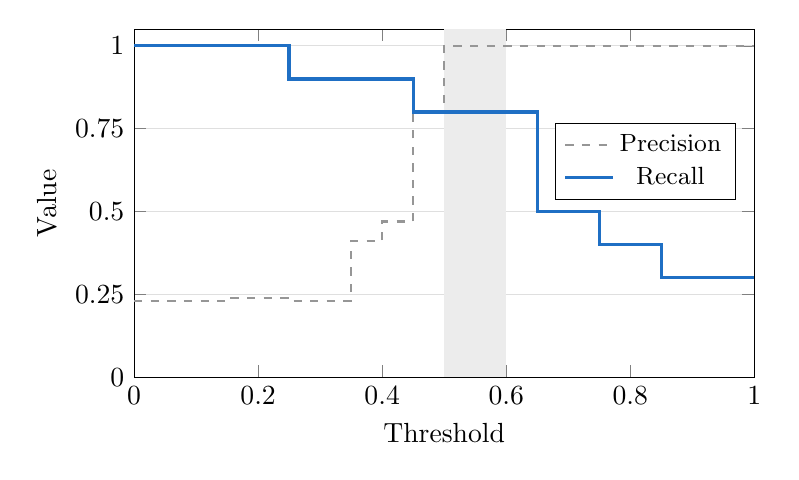
\begin{tikzpicture}
\begin{axis}[
  width=0.78\linewidth, height=6cm,
  xmin=0, xmax=1, ymin=0, ymax=1.05,
  xlabel={Threshold}, ylabel={Value},
  xtick={0,0.2,0.4,0.6,0.8,1}, ytick={0,0.25,0.5,0.75,1},
  ymajorgrids, grid style={gray!25},
  legend style={at={(0.97,0.62)},anchor=east,font=\small},
]
\fill[gray!15] (axis cs:0.5,0) rectangle (axis cs:0.6,1.05);
\addplot[const plot, thick, color=paper, dashed] coordinates {
 (0,0.23) (0.05,0.23) (0.10,0.23) (0.15,0.24) (0.20,0.24) (0.25,0.23) (0.30,0.23) (0.35,0.41)
 (0.40,0.47) (0.45,0.80) (0.50,1) (0.55,1) (0.60,1) (0.65,1) (0.70,1) (0.75,1) (0.80,1)
 (0.85,1) (0.90,1) (0.95,1) (1,1)};
\addplot[const plot, very thick, color=ours] coordinates {
 (0,1) (0.05,1) (0.10,1) (0.15,1) (0.20,1) (0.25,0.9) (0.30,0.9) (0.35,0.9) (0.40,0.9)
 (0.45,0.8) (0.50,0.8) (0.55,0.8) (0.60,0.8) (0.65,0.5) (0.70,0.5) (0.75,0.4) (0.80,0.4)
 (0.85,0.3) (0.90,0.3) (0.95,0.3) (1,0.3)};
\legend{Precision, Recall}
\end{axis}
\end{tikzpicture}
\caption{Precision and recall over all 44 labelled clusters as the threshold varies; shaded: the
range with precision 1.00 and the highest recall (0.80).}
\label{fig:sweep}
\end{figure}

On the unlabelled 13.4-hour capture, 322 of 1{,}910 clusters (27{,}860 reports) score at least 0.5,
mostly from \pass{intercept\_path} (147) and \pass{access} (145). Some of these come from our own
scenario programs, which ran during the capture. No precision is claimed for this data set because
it is not labelled.

% ================================================================ 10
\section{Limitations and threats to validity}

\begin{itemize}
  \item \textbf{Circular evaluation.} The scenario labels and the score rules both build on the
  same notion of a privilege boundary, so high precision partly confirms that the context is
  captured correctly rather than that the score predicts real-world bugs.
  \item \textbf{Small, synthetic ground truth.} 44 labelled clusters from constructed scenarios;
  three passes are not scored at all.
  \item \textbf{Stand-in workloads.} Table~\ref{tab:t3} uses five open-source programs instead of
  SPEC CPU~2017, and Browserbench was not run.
  \item \textbf{Different hardware.} Our VM uses a different CPU and more vCPUs than the paper's
  System~A; we therefore compare overhead ratios, not absolute times. The memcpy result also
  depends on CPU features (Section~\ref{sec:bugs}).
  \item \textbf{Single capture.} The 13.4-hour capture covers one developer VM and includes our
  own benchmark and scenario runs.
\end{itemize}

% ================================================================ 11
\section{Conclusion and future work}

OS-Sanitizer's published results hold on independent hardware: the artifact builds, all passes
detect their targets, and the overhead ranking matches both of the paper's benchmark tables. We
fixed a CPU-dependent detection bug and found a pass interaction bug. Kernel-captured context and
automated clustering reduce a night of system-wide reports from 207{,}854 lines to 1{,}910 items,
and to 1{,}034 for the ERROR/WARN reports analysts read, which addresses the paper's usability
problem directly. A transparent score built on that context separates safe from exploitable
variants of the same code in labelled scenarios.

Next steps:
\begin{enumerate}
  \item label clusters from a longer real capture, by two people independently, and report their
  agreement;
  \item validate the stack depth by measuring cluster purity on that labelled data;
  \item capture the source location of copied data so the memory-copy passes can be scored;
  \item replace the hand-set weights with logistic regression evaluated on held-out data;
  \item locate and fix the \pass{intercept\_path}/\pass{sec\_file\_open} interaction;
  \item prototype LSM enforcement for one pass, in audit mode first, in an isolated VM.
\end{enumerate}

% ================================================================ refs
\begin{thebibliography}{9}\small
\bibitem{ossan} A.~Crump, S.~Sihag, F.~Bauckholt, K.~Hassler, and T.~Holz, ``OS-Sanitizer:
System-wide latent defect inference in Linux applications,'' in \emph{Proc.\ 35th USENIX Security
Symposium}, 2026, pp.~2763--2782.
\bibitem{artifact} OS-Sanitizer open-source artifact.
\url{https://github.com/os-sanitizer/os-sanitizer}
\bibitem{weipu} J.~Wei and C.~Pu, ``TOCTTOU vulnerabilities in UNIX-style file systems: An
anatomical study,'' in \emph{Proc.\ USENIX FAST}, 2005.
\bibitem{fontana} F.~A.~Fontana \emph{et al.}, ``Antipattern and code smell false positives:
Preliminary conceptualization and classification,'' in \emph{Proc.\ IEEE SANER}, 2016.
\bibitem{heckman} S.~Heckman and L.~Williams, ``A systematic literature review of actionable alert
identification techniques for automated static code analysis,'' \emph{Information and Software
Technology}, vol.~53, no.~4, pp.~363--387, 2011.
\bibitem{kremenek} T.~Kremenek and D.~Engler, ``Z-Ranking: Using statistical analysis to counter the
impact of static analysis approximations,'' in \emph{Proc.\ SAS}, 2003.
\bibitem{raducu} R.~Raducu, R.~J.~Rodr\'iguez, and P.~Alvarez, ``Defense and attack techniques against
file-based TOCTOU vulnerabilities: A systematic review,'' \emph{IEEE Access}, vol.~10,
pp.~21742--21758, 2022.
\end{thebibliography}

\end{document}
